% Units of Z[sqrt 2] on the hyperbolas x^2-2y^2=+-1.
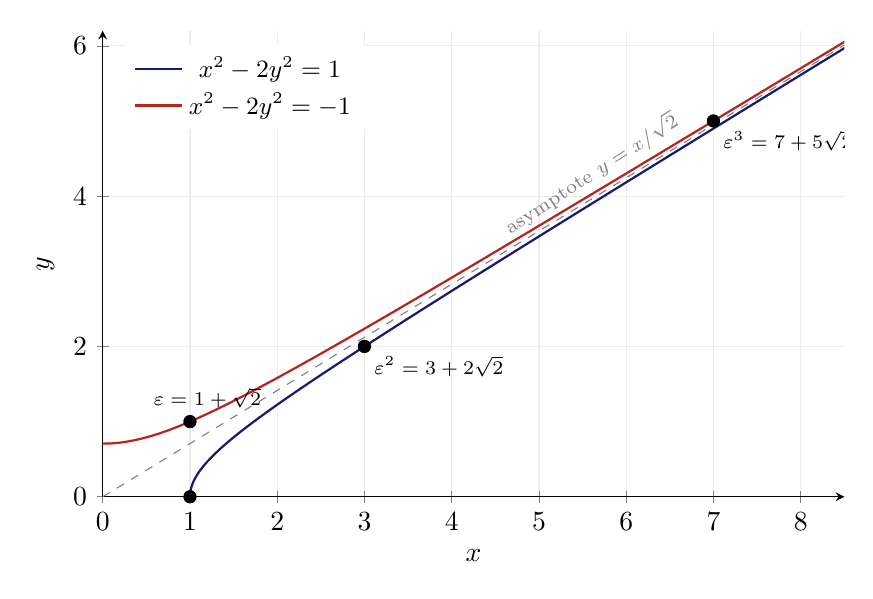
\begin{tikzpicture}
\begin{axis}[width=11cm,height=7.5cm,xmin=0,xmax=8.5,ymin=0,ymax=6.2,
    axis lines=left,xlabel={$x$},ylabel={$y$},grid=major,grid style={gray!15},
    legend style={at={(0.03,0.97)},anchor=north west,font=\small,draw=none,fill=white}]
  \addplot[domain=0:2.9,samples=80,MidnightBlue,thick] ({cosh(x)},{sinh(x)/sqrt(2)});
  \addlegendentry{$x^2-2y^2=1$}
  \addplot[domain=0:2.9,samples=80,BrickRed,thick] ({sinh(x)},{cosh(x)/sqrt(2)});
  \addlegendentry{$x^2-2y^2=-1$}
  \addplot[only marks,mark=*,mark size=2.2pt,black] coordinates {(1,0) (1,1) (3,2) (7,5)};
  \node[below right,font=\scriptsize] at (axis cs:1,0) {$1$};
  \node[above,font=\scriptsize] at (axis cs:1.2,1.05) {$\varepsilon=1+\sqrt2$};
  \node[below right,font=\scriptsize] at (axis cs:3,2) {$\varepsilon^2=3+2\sqrt2$};
  \node[below right,font=\scriptsize] at (axis cs:7,5) {$\varepsilon^3=7+5\sqrt2$};
  \addplot[domain=0:8.5,gray,dashed] {x/sqrt(2)}; \node[gray,font=\scriptsize,rotate=33] at (axis cs:5.6,4.3) {asymptote $y=x/\sqrt2$};
\end{axis}
\end{tikzpicture}
